%% journal_paper.tex
%% TrustVault: Trustless Academic Credential Verification on ICP
%% IEEE Journal Style — compile with pdflatex (twice for refs)

\documentclass[journal]{IEEEtran}

%% ---------- packages ----------
\usepackage[T1]{fontenc}
\usepackage[utf8]{inputenc}
\usepackage{amsmath,amssymb}
\usepackage{graphicx}
\usepackage{booktabs}
\usepackage{array}
\usepackage{multirow}
\usepackage{url}
\usepackage{hyperref}
\hypersetup{colorlinks=false, pdfborder={0 0 0}}
\usepackage{tikz}
\usetikzlibrary{
  arrows.meta, positioning, shapes.geometric,
  shapes.misc, fit, calc,
  decorations.pathreplacing, backgrounds
}
\usepackage{pgfplots}
\pgfplotsset{compat=1.18}
\usepackage{pgfplotstable}
\usepackage{listings}
\lstset{
  basicstyle=\ttfamily\scriptsize,
  breaklines=true,
  frame=single,
  captionpos=b
}
\usepackage{enumitem}
\usepackage{balance}

%% ---------- custom colours ----------
\definecolor{icpblue}{RGB}{59,130,246}
\definecolor{icpgreen}{RGB}{34,197,94}
\definecolor{icpyellow}{RGB}{234,179,8}
\definecolor{icppurple}{RGB}{139,92,246}
\definecolor{icpred}{RGB}{239,68,68}
\definecolor{icpgray}{RGB}{100,116,139}
\definecolor{lightblue}{RGB}{219,234,254}
\definecolor{lightgreen}{RGB}{220,252,231}
\definecolor{lightyellow}{RGB}{254,249,195}
\definecolor{lightpurple}{RGB}{237,233,254}

% =========================================================
\begin{document}

\title{TrustVault: A Fully On-Chain, Trustless Academic Credential Verification System on the Internet Computer Protocol}

\author{
  Varun~Gudamsetti
  \and
  Shruti~Jadon
  \thanks{V.~Gudamsetti and S.~Jadon are with the Department of Computer Science and Engineering, PES University, Bengaluru, Karnataka, India. E-mail: varun.gudamsetti@pes.edu, shrutijadon@pes.edu.}
}

\markboth{IEEE Journal — March 2026}%
{Gudamsetti and Jadon: TrustVault}

\maketitle

% =========================================================
\begin{abstract}
Fake academic credentials are a growing problem that affects employers, universities, and students worldwide. Current verification methods are either manual and slow, or depend on centralized databases that can be tampered with or go offline. Blockchain-based solutions have been proposed, but public blockchains like Ethereum charge high fees for every write operation, and permissioned blockchains like Hyperledger Fabric require trust in consortium members. In all existing systems, the verification website itself runs on a regular web server — a single point of failure.

This paper presents \textbf{TrustVault}, an academic credential verification system that is \emph{fully on-chain} — both the data and the user-facing website live on the Internet Computer Protocol (ICP) blockchain. TrustVault uses an incremental Merkle tree combined with ICP's \emph{Certified Variables} (values signed by the subnet's threshold BLS key) so that anyone can verify a credential mathematically, without trusting any single server or institution. We deploy TrustVault on the ICP mainnet and run a comprehensive benchmark suite. Our results show: single-certificate issuance in about 1.9 seconds, verification queries as fast as 177 milliseconds, parallel throughput up to 7.3 certificates per second, concurrent mixed-workload throughput of 13.6 operations per second with zero errors, block finality of 2.36 seconds (p99 under 3 seconds), and an issuance cost of approximately \$0.001 per certificate — orders of magnitude cheaper than Ethereum.
\end{abstract}

\begin{IEEEkeywords}
Blockchain, Internet Computer Protocol, Academic Credentials, Merkle Tree, Certified Variables, Zero-Trust Verification, Motoko, Threshold BLS Signatures
\end{IEEEkeywords}

% =========================================================
\section{Introduction}
\label{sec:intro}

Academic credential fraud is a serious and growing problem. Studies estimate that a significant portion of job applications contain misrepresented qualifications~\cite{chahal2021credential}. When an employer wants to check whether a candidate truly holds a claimed degree, the typical process involves contacting the issuing university, waiting days for a response, and trusting that the reply is genuine. This manual approach is slow, expensive, and does not scale to global hiring.

Several digital alternatives exist, but each has significant drawbacks:

\begin{itemize}[leftmargin=*]
  \item \textbf{Centralized registries} (e.g., government databases, third-party services like the National Student Clearinghouse) are convenient, but if the registry goes offline, gets hacked, or is corrupted, verification becomes impossible. The verifier must trust the registry operator completely.
  \item \textbf{Public blockchains like Ethereum}~\cite{buterin2014ethereum} offer strong tamper resistance, but writing a single credential record costs several dollars in gas fees, making it impractical for universities that issue thousands of degrees annually. Moreover, the verification interface (website) still runs on a regular web server.
  \item \textbf{Permissioned blockchains like Hyperledger Fabric}~\cite{androulaki2018fabric} reduce cost but reintroduce trust: one must trust all consortium members. If the consortium is compromised, so are the credentials.
  \item \textbf{Hybrid systems} that store only hashes on-chain while keeping actual data on a separate server effectively bring back centralization through the back door.
\end{itemize}

A key observation is that \emph{none} of the above systems serve the verification interface from the blockchain itself. The user-facing website is always hosted on a traditional cloud server (AWS, GCP, etc.), which means it can be tampered with, taken down, or censored independently of the on-chain data.

The \textbf{Internet Computer Protocol (ICP)}~\cite{hanke2018dfinity}, developed by the DFINITY Foundation, offers a fundamentally different approach. ICP is a decentralized compute platform where smart contracts — called \emph{canisters} — run as WebAssembly modules replicated across independent \emph{subnets} of geographically distributed nodes. Three ICP features are especially relevant:

\begin{enumerate}
  \item \textbf{On-chain web serving}: Canisters can directly respond to HTTP requests, so the verification website itself lives on the blockchain — no cloud hosting needed.
  \item \textbf{Certified Variables}: A built-in API that lets a canister commit a 32-byte value (such as a Merkle root) which the subnet's threshold BLS key then signs. Any client can verify this signature using the publicly known subnet key, without trusting the canister or any individual node.
  \item \textbf{Low cost}: Storing data on ICP costs a fraction of a cent, making it practical to store hundreds of thousands of credentials.
\end{enumerate}

\subsection{Contributions}

This paper makes the following contributions:

\begin{enumerate}
  \item We design and implement \textbf{TrustVault}, the first fully on-chain academic credential verification system — both frontend and backend — deployed on a public blockchain mainnet.
  \item We integrate an \textbf{incremental binary Merkle tree} with ICP's Certified Variables to create a tamper-evident credential registry that costs O($\log n$) per insert.
  \item We describe a \textbf{trustless verification protocol} in which a verifier who knows only the ICP root public key can independently confirm any credential without contacting the issuing university.
  \item We present a \textbf{comprehensive performance evaluation} on ICP mainnet, covering issuance latency, verification latency, throughput, scalability, concurrent mixed workloads, block finality, and cost — all measured on a live production deployment.
  \item We provide a \textbf{cross-platform comparison} with Ethereum PoS and Hyperledger Fabric using published benchmarks and citations.
\end{enumerate}

\subsection{Paper Organization}

The rest of this paper is organized as follows. Section~\ref{sec:background} covers background on credential fraud and blockchain approaches. Section~\ref{sec:related} discusses related work in detail. Section~\ref{sec:architecture} presents the system architecture and design decisions. Section~\ref{sec:merkle} explains the Merkle tree and trustless verification mechanism. Section~\ref{sec:impl} describes the implementation. Section~\ref{sec:eval} presents the experimental evaluation. Section~\ref{sec:discussion} discusses limitations and practical considerations. Section~\ref{sec:conclusion} concludes and outlines future work.

% =========================================================
\section{Background}
\label{sec:background}

This section provides the necessary context on academic credential fraud, blockchain technology, and the Internet Computer Protocol.

\subsection{The Problem of Academic Credential Fraud}

Academic credential fraud takes two main forms: \emph{fabricated credentials} (entirely fake degrees from diploma mills or forged documents) and \emph{misrepresented credentials} (genuine degrees with inflated grades, false dates, or fabricated distinctions). Reports suggest that roughly one in five professional job applications in certain regions contain at least one credential misrepresentation~\cite{chahal2021credential}.

The traditional verification process works as follows: an employer contacts the university's registrar office, provides the candidate's name and claimed degree, and waits for a manual confirmation. This process can take anywhere from a few days to several weeks, costs money, and fundamentally relies on the employer trusting the registrar's response. If the registrar's database is compromised or if the communication channel is intercepted, there is no way for the employer to independently verify the answer.

\subsection{Blockchain Basics}

A blockchain is a distributed ledger — a shared database maintained by multiple independent nodes that agree on its contents through a \emph{consensus protocol}. Once data is written to a blockchain (``committed''), it is extremely difficult to change without being detected, because every subsequent block cryptographically references the previous one.

Two types of blockchains are relevant:
\begin{itemize}[leftmargin=*]
  \item \textbf{Public (permissionless) blockchains} like Bitcoin and Ethereum allow anyone to join the network and validate transactions. They offer strong decentralization but can be expensive (gas fees) and slow (Ethereum PoS finality takes about 12--24 seconds~\cite{buterin2020eth2}).
  \item \textbf{Permissioned blockchains} like Hyperledger Fabric~\cite{androulaki2018fabric} restrict participation to known entities. They achieve higher throughput (up to 3,500 transactions per second) and lower cost, but the verifier must trust the consortium that operates the chain.
\end{itemize}

\subsection{Internet Computer Protocol (ICP)}
\label{subsec:icp}

The Internet Computer Protocol~\cite{hanke2018dfinity} is a public blockchain that takes a fundamentally different approach. Instead of running a single global chain, ICP operates multiple independent \emph{subnets}, each consisting of 13--40 geographically distributed \emph{replica nodes} operated by independent entities. Each subnet runs its own consensus protocol and hosts a set of smart contracts called \emph{canisters}.

\subsubsection{Consensus}
ICP uses a four-phase Byzantine Fault Tolerant (BFT) consensus protocol~\cite{hanke2018dfinity}:
\begin{enumerate}
  \item \textbf{Random Beacon}: A threshold BLS signature~\cite{boneh2001bls} over the previous round's beacon generates an unpredictable, publicly verifiable random number.
  \item \textbf{Block Making}: The beacon determines a ranking of block-maker candidates. The highest-ranked available node proposes a block.
  \item \textbf{Notarization}: At least two-thirds of subnet nodes sign the proposed block using threshold BLS shares.
  \item \textbf{Finalization}: Once a round has exactly one notarized block, it is finalized by another threshold signature.
\end{enumerate}

This achieves finality in approximately 1--3 seconds, which is significantly faster than Ethereum's 12--24 seconds and orders of magnitude faster than Bitcoin's 60 minutes.

\subsubsection{Canisters}
A canister is a WebAssembly module with its own persistent memory, similar to a container in cloud computing but replicated across an entire subnet. Canisters support two types of calls:
\begin{itemize}[leftmargin=*]
  \item \textbf{Update calls} modify the canister's state, go through consensus, and finalize in approximately 2 seconds. They cost a small amount of ``cycles'' (ICP's unit of computation).
  \item \textbf{Query calls} are read-only operations that execute on a single replica without going through consensus. They return in under 500 milliseconds and are \emph{free} for the caller.
\end{itemize}

\subsubsection{Chain-Key Cryptography and Certified Variables}
Every ICP subnet holds a \emph{threshold BLS key pair}~\cite{boneh2001bls}: the private key is secret-shared among the subnet's nodes using a Distributed Key Generation (DKG) protocol, so no single node ever holds the full private key. The corresponding public key is known to every client.

\emph{Certified Variables} are a built-in feature that lets a canister store a 32-byte value (e.g., a Merkle root) via the \texttt{CertifiedData.set()} API. After the next consensus round, the subnet collectively signs this value as part of the \emph{state tree}. When a client makes a query, the response can include a \emph{certificate} — the BLS-signed state tree — that the client can verify using the subnet's public key. This means:
\begin{itemize}[leftmargin=*]
  \item The client does not need to trust the individual node that answered the query.
  \item The client does not need to trust the canister's code.
  \item Verification is purely mathematical: check the BLS signature against the known public key.
\end{itemize}

\subsubsection{On-Chain Web Serving}
Unlike Ethereum or Bitcoin, ICP canisters can respond directly to HTTP requests. A special ``asset canister'' can host an entire website (HTML, JavaScript, CSS, images) on-chain. The ICP HTTP gateway~\cite{dfinity2023httpgateway} translates browser requests into canister query calls and returns the responses. Certified HTTP headers ensure that even the served web pages are cryptographically authenticated — a browser-level extension or middleware can verify that the page content was not tampered with in transit. This eliminates the need for any external web hosting and ensures that even the user interface is tamper-resistant.

\subsubsection{Network Nervous System and Governance}
ICP is governed by the \emph{Network Nervous System} (NNS), an on-chain decentralized autonomous organization (DAO). The NNS controls subnet creation, node onboarding, protocol upgrades, and other governance decisions. All changes require community approval through a proposal-and-voting mechanism where ICP token holders stake tokens as ``neurons'' with voting power. This means no single entity — including the DFINITY Foundation — can unilaterally change the platform. Subnet public keys are also registered and verifiable through the NNS, which forms the root of trust for the entire Certified Variables mechanism.

\subsubsection{Cycles and Cost Model}
Computation on ICP is paid for using \emph{cycles}, which are pegged to the Swiss Franc at a fixed exchange rate (1 trillion cycles = 1 XDR $\approx$ \$1.35). Canister operators ``top up'' their canisters with cycles, and each operation (update call, memory storage, network bandwidth) consumes a known amount. Critically, \emph{query calls are free} for the caller — the canister operator absorbs the cost. This means that credential verification in TrustVault costs nothing to the employer or verifier, regardless of how many queries they make. Issuance (an update call) costs approximately 590,000 cycles per call, which translates to roughly \$0.001 per certificate at current exchange rates.

% =========================================================
\section{Related Work}
\label{sec:related}

This section reviews prior work on blockchain-based credential systems and positions TrustVault relative to the state of the art.

\subsection{MIT Digital Diplomas and Blockcerts}
In 2017, MIT Media Lab pioneered the idea of anchoring diploma hashes on the Bitcoin blockchain~\cite{grech2017blockchain}. The Blockcerts open standard defines a JSON-LD schema for digital credentials and stores a hash of each credential as a Bitcoin transaction. However, Bitcoin is not programmable — there is no smart contract logic on Bitcoin — so the verification frontend runs on a traditional web server maintained by MIT. If that server goes down or is compromised, verification becomes impossible even though the hash remains on Bitcoin. Additionally, Bitcoin transaction fees (several dollars per transaction) make it expensive to issue credentials at scale.

\subsection{EduCTX}
Turkanovi\'{c} et al.~\cite{turk2018eductx} proposed EduCTX, a blockchain platform specifically designed for higher education credit transfer across the European Higher Education Area. EduCTX uses a permissioned blockchain based on the Ark platform, where consortium members (universities) act as validators. While this approach achieves good performance, it requires trust in the participating institutions — if a subset of consortium members collude, they could forge or alter credential records. The verification interface is also centralized.

\subsection{Ethereum-Based Credential Systems}
Several projects have used Ethereum smart contracts to manage academic credentials~\cite{lizcano2020blockchain}. The typical approach stores a SHA-256 hash of each credential on Ethereum while keeping the full credential data off-chain (on IPFS, a university server, or a cloud database). This is a pragmatic choice given Ethereum's high gas costs, but it reintroduces centralization: if the off-chain storage goes down, the credential data is lost even though its hash remains on Ethereum. Gas costs for a credential write operation range from \$0.20 to \$2.00 depending on network congestion~\cite{wood2014ethereum}.

\subsection{W3C Verifiable Credentials}
The W3C Verifiable Credentials Data Model~\cite{w3c2022vc} provides a standardized format for expressing credentials digitally. It defines the concepts of Issuer, Holder, and Verifier, along with cryptographic proof mechanisms. However, the W3C standard is a \emph{data format}, not a platform — it does not specify where or how credentials should be stored. Most implementations use either permissioned blockchains or centralized registries as the storage backend.

\subsection{Summary and Gap Analysis}

Table~\ref{tab:related_comparison} summarizes the key differences between existing approaches and TrustVault.

\begin{table*}[t]
\caption{Comparison of Credential Verification Systems}
\label{tab:related_comparison}
\centering\small\renewcommand{\arraystretch}{1.2}
\begin{tabular}{@{}lcccccc@{}}
\toprule
\textbf{System} & \textbf{On-Chain Data} & \textbf{On-Chain UI} & \textbf{Trustless} & \textbf{Low Cost} & \textbf{Mainnet Deployed} & \textbf{Benchmarked} \\
\midrule
Blockcerts / MIT~\cite{grech2017blockchain}        & Hash only  & No  & No  & No (\$2+/tx)  & Yes (Bitcoin) & No \\
EduCTX~\cite{turk2018eductx}                       & Full       & No  & No  & Yes           & No            & Limited \\
Ethereum hash systems~\cite{lizcano2020blockchain}  & Hash only  & No  & Partial & No (\$0.20+) & Yes (Ethereum) & No \\
Hyperledger Fabric~\cite{androulaki2018fabric}      & Full       & No  & No  & Yes           & Private       & Yes \\
W3C VC~\cite{w3c2022vc}                            & Varies     & No  & Varies & Varies       & Varies        & No \\
Self-Sovereign Identity~\cite{allen2016decentralized} & Varies  & No  & Partial & Varies       & Varies        & No \\
\textbf{TrustVault (this work)}                     & \textbf{Full} & \textbf{Yes} & \textbf{Yes} & \textbf{Yes (\$0.001)} & \textbf{Yes (ICP)} & \textbf{Yes} \\
\bottomrule
\end{tabular}
\end{table*}

The key gap that TrustVault fills: no prior system (a) stores the complete credential record on a public blockchain, (b) serves the verification interface from the blockchain itself, (c) provides mathematically verifiable proofs via Certified Variables, and (d) has been benchmarked on a live mainnet deployment with published results.

\subsection{Self-Sovereign Identity and Decentralized Identifiers}

The Self-Sovereign Identity (SSI) movement~\cite{allen2016decentralized} advocates for individuals to own and control their own identity data, without depending on any central authority. Decentralized Identifiers (DIDs) and Verifiable Credentials (VCs) are the technical building blocks of SSI. While TrustVault shares the goal of eliminating trust in central authorities, it takes a different approach: instead of giving each individual control over their credential data, TrustVault stores credentials on a public blockchain where anyone can verify them. The two approaches are complementary — a future version of TrustVault could wrap its credentials in W3C VC format and associate them with DIDs.

\subsection{Blockchain Timestamping for Academic Documents}

Gipp et al.~\cite{gipp2015decentralized} proposed using Bitcoin transactions to timestamp academic documents, providing proof of existence at a particular point in time. This is a lighter-weight approach than full credential storage, but it only proves that a document existed at a certain time — it does not prove who issued it, whether it has been revoked, or whether the content is authentic. TrustVault goes further by storing the full credential record and providing cryptographic verification of both authenticity and provenance.

\subsection{Systematic Reviews}

Nzaou et al.~\cite{nzaou2022credential} conducted a systematic review of 47 blockchain-based credential verification systems published between 2017 and 2022. Their key findings align with our gap analysis: most systems store only hashes on-chain, none serve the verification UI from the blockchain, and very few provide quantitative performance benchmarks on a live deployment. TrustVault addresses all three gaps.

% =========================================================
\section{System Architecture}
\label{sec:architecture}

TrustVault consists of two ICP canisters deployed on the public mainnet: a \emph{backend canister} written in Motoko (ICP's native language) that stores credentials and handles business logic, and a \emph{frontend canister} (an asset canister) that hosts a React single-page application served directly over HTTPS from the blockchain.

\subsection{High-Level Architecture}

Fig.~\ref{fig:sysarch} shows the overall system architecture. The three user roles are:

\begin{itemize}[leftmargin=*]
  \item \textbf{University (Issuer)}: A registered institution that issues credentials by calling the \texttt{issueCertificate} update function.
  \item \textbf{Student (Holder)}: The recipient of a credential, who can view their credentials through the portal.
  \item \textbf{Verifier (Employer)}: Any party that wants to verify a credential by calling the \texttt{verifyCertificate} query function.
\end{itemize}

All three roles interact with the system through the on-chain React frontend, which communicates with the backend canister using auto-generated Candid type bindings (Candid is ICP's interface description language, similar to Protocol Buffers).

\begin{figure}[t]
\centering
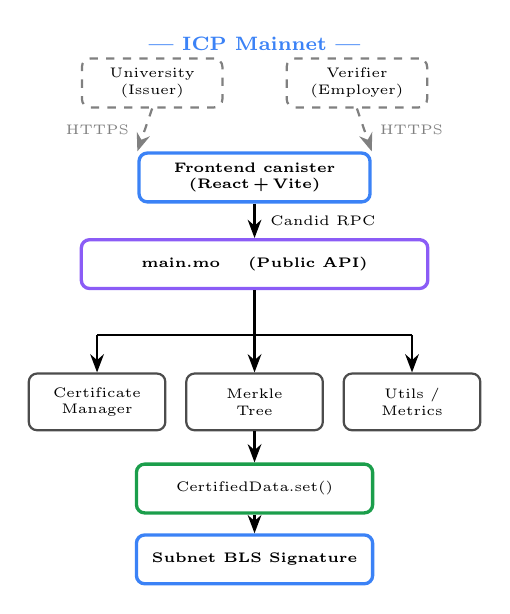
\begin{tikzpicture}[
  actor/.style={rectangle, rounded corners=3pt, draw=gray, dashed, thick,
                minimum height=0.62cm, minimum width=1.65cm, text width=1.55cm,
                font=\tiny, align=center},
  fe/.style={rectangle, rounded corners=3pt, draw=icpblue, very thick,
             minimum height=0.62cm, minimum width=2.8cm, text width=2.7cm,
             font=\tiny\bfseries, align=center},
  api/.style={rectangle, rounded corners=3pt, draw=icppurple, very thick,
              minimum height=0.62cm, minimum width=4.4cm,
              font=\tiny\bfseries, align=center},
  mod/.style={rectangle, rounded corners=3pt, draw=black!70, thick,
              minimum height=0.72cm, minimum width=1.6cm, text width=1.5cm,
              font=\tiny, align=center},
  certd/.style={rectangle, rounded corners=3pt, draw=icpgreen!80!black, very thick,
                minimum height=0.62cm, minimum width=3.0cm,
                font=\tiny, align=center},
  bls/.style={rectangle, rounded corners=3pt, draw=icpblue, very thick,
              minimum height=0.62cm, minimum width=3.0cm,
              font=\tiny\bfseries, align=center},
  arr/.style={-Stealth, thick},
  every node/.style={font=\tiny}
]
  \node[mod] (cm) at (0.0, 0.0) {Certificate\\Manager};
  \node[mod] (mt) at (2.0, 0.0) {Merkle\\Tree};
  \node[mod] (ut) at (4.0, 0.0) {Utils /\\Metrics};
  \node[api] (main) at (2.0, 1.75) {\textbf{main.mo} \quad (Public API)};
  \node[fe] (front) at (2.0, 2.85) {Frontend canister (React\,+\,Vite)};
  \node[actor] (uni) at (0.7, 4.05) {University\\(Issuer)};
  \node[actor] (ver) at (3.3, 4.05) {Verifier\\(Employer)};
  \node[font=\scriptsize\bfseries, icpblue] at (2.0, 4.55) {--- ICP Mainnet ---};
  \node[certd] (cd)  at (2.0, -1.10) {CertifiedData.set()};
  \node[bls]   (sub) at (2.0, -2.00) {Subnet BLS Signature};
  \draw[arr, dashed, gray] (uni.south) -- node[left=2pt, font=\tiny, pos=0.5]{HTTPS} (front.north west);
  \draw[arr, dashed, gray] (ver.south) -- node[right=2pt, font=\tiny, pos=0.5]{HTTPS} (front.north east);
  \draw[arr] (front.south) -- node[right=2pt, font=\tiny]{Candid RPC} (main.north);
  \draw[thick] (main.south) -- (2.0, 0.85);
  \draw[thick] (0.0, 0.85)  -- (4.0, 0.85);
  \draw[arr]   (0.0, 0.85)  -- (cm.north);
  \draw[arr]   (2.0, 0.85)  -- (mt.north);
  \draw[arr]   (4.0, 0.85)  -- (ut.north);
  \draw[arr] (mt.south) -- (cd.north);
  \draw[arr] (cd.south) -- (sub.north);
\end{tikzpicture}
\caption{TrustVault system architecture. Users connect via HTTPS to the on-chain frontend, which routes requests to the backend canister. The Merkle tree root is BLS-signed by the ICP subnet.}
\label{fig:sysarch}
\end{figure}

\subsection{Backend Modules}

The backend canister is organized into five Motoko modules:

\begin{enumerate}
  \item \textbf{main.mo} — The public actor that exposes the API: \texttt{issueCertificate}, \texttt{revokeCertificate}, \texttt{verifyCertificate}, \texttt{registerUniversity}, and various query functions.
  \item \textbf{CertificateManager.mo} — Handles certificate creation, hash computation, and verification logic.
  \item \textbf{MerkleTree.mo} — Implements the incremental binary Merkle tree with O($\log n$) insertion.
  \item \textbf{Utils.mo} — Provides SHA-256 hashing and hex encoding utilities.
  \item \textbf{PerformanceMetrics.mo} — Records on-chain telemetry (operation latencies, counts, percentiles) for monitoring.
\end{enumerate}

\subsection{Certificate Schema}

Each credential is stored as a Motoko record with the fields shown in Table~\ref{tab:schema}.

\begin{table}[h]
\caption{Certificate Record Schema}
\label{tab:schema}
\centering\small\renewcommand{\arraystretch}{1.1}
\begin{tabular}{@{}lll@{}}
\toprule
\textbf{Field} & \textbf{Type} & \textbf{Description} \\
\midrule
\texttt{certificate\_id}    & Text   & Unique identifier \\
\texttt{certificate\_hash}  & Text   & SHA-256 of core fields \\
\texttt{issuer}             & Record & University name, canister ID, URL \\
\texttt{recipient}          & Record & Student name, ID, principal \\
\texttt{credential}         & Record & Degree type, major, GPA, dates \\
\texttt{is\_revoked}        & Bool   & Revocation flag \\
\texttt{block\_timestamp}   & Int64  & Consensus-set nanosecond timestamp \\
\texttt{schema\_version}    & Text   & Currently ``1.0'' \\
\bottomrule
\end{tabular}
\end{table}

The \texttt{certificate\_hash} is computed as $H = \text{SHA-256}(\texttt{id} \| \texttt{issuer} \| \texttt{name} \| \texttt{student\_id} \| \texttt{degree} \| \texttt{major} \| \texttt{date})$. This hash becomes a leaf in the Merkle tree.

\subsection{Access Control}

Access control uses ICP \emph{Principals} — cryptographic identities derived from Ed25519 key pairs. Each user (university, student, verifier) has a unique Principal. The system maintains a registry of university Principals; only registered universities may call \texttt{issueCertificate} or \texttt{revokeCertificate}. The \texttt{verifyCertificate} function is a public \emph{query call}, meaning anyone can verify any credential for free without authentication.

\subsection{Frontend Design}

The frontend is a React single-page application built with Vite and hosted entirely inside an ICP asset canister. It consists of three portals:

\begin{itemize}[leftmargin=*]
  \item \textbf{University Portal}: Allows registered universities to issue new credentials by filling in student information and clicking ``Issue.'' The portal calls the \texttt{issueCertificate} update function and displays the resulting certificate hash and ID.
  \item \textbf{Student Portal}: Allows students to view their credentials by entering their student ID. The portal calls \texttt{getCertificatesByStudent} (a query function) and displays all matching credentials.
  \item \textbf{Verification Portal}: Allows any employer or third party to verify a credential by entering its certificate ID. The portal calls \texttt{verifyCertificate} (a query function), receives the Merkle proof and verification result, and displays a clear pass/fail status along with the full credential details.
\end{itemize}

The frontend communicates with the backend through auto-generated Candid type bindings (Candid is ICP's interface description language, analogous to Protocol Buffers or GraphQL schemas). These bindings ensure type safety: the JavaScript frontend code is guaranteed to match the Motoko backend API at compile time.

\subsection{Workflow}

The typical workflow for credential issuance and verification is:

\begin{enumerate}
  \item \textbf{University registers}: A university calls \texttt{registerUniversity(name)} with its Principal. This is a one-time setup step.
  \item \textbf{University issues credential}: The university fills in the student's information in the University Portal and clicks ``Issue.'' The backend creates the certificate record, computes its SHA-256 hash, inserts the hash into the Merkle tree, and commits the new root via \texttt{CertifiedData.set()}.
  \item \textbf{Credential becomes verifiable}: Within one consensus round (about 2 seconds), the new Merkle root is BLS-signed by the subnet. The credential is now independently verifiable.
  \item \textbf{Employer verifies}: An employer enters the certificate ID in the Verification Portal. The query returns the certificate data, the Merkle proof, and the certified root. The frontend (or any client) can independently verify the proof chain.
  \item \textbf{Revocation (if needed)}: If a credential needs to be revoked (e.g., academic misconduct discovered), the university calls \texttt{revokeCertificate}. The Merkle tree is rebuilt and the new root invalidates all previous proofs within 2 seconds.
\end{enumerate}

% =========================================================
\section{Merkle Tree and Trustless Verification}
\label{sec:merkle}

This section explains how TrustVault achieves trustless verification — a process where the verifier does not need to trust any server, institution, or even the canister code.

\subsection{Incremental Binary Merkle Tree}

All certificate hashes are stored as leaves of a complete binary Merkle tree~\cite{merkle1989certified}. The tree is implemented as a flat array of size $2C - 1$, where $C$ is the smallest power of two greater than or equal to the number of certificates. Leaf $i$ is at array index $C - 1 + i$, and the root is at index 0.

Each internal node stores the hash of its two children:
\begin{equation}
  \texttt{nodes}[j] = \text{SHA-256}(\texttt{nodes}[2j+1] \;\|\; \texttt{nodes}[2j+2])
  \label{eq:merkle}
\end{equation}

\textbf{Insertion} (O($\log n$)): When a new certificate is issued, its hash is placed at the next available leaf position. Then, only the nodes along the path from that leaf to the root are recomputed — a sequence of $\lceil\log_2 n\rceil$ hash operations. The updated 32-byte root is committed via \texttt{CertifiedData.set()}.

\textbf{Proof generation} (O($\log n$)): To prove that a certificate exists in the tree, the system returns the list of \emph{sibling hashes} along the path from the leaf to the root. The verifier can recompute the root from these siblings and compare it to the certified root.

\textbf{Revocation} (O($n$)): When a certificate is revoked, its \texttt{is\_revoked} flag is set to true, and the entire Merkle tree is rebuilt. The new root is committed via \texttt{CertifiedData.set()}, invalidating all previous proofs within one consensus round (about 2 seconds).

Fig.~\ref{fig:merkle} illustrates the tree structure and a sample proof path.

\begin{figure}[t]
\centering
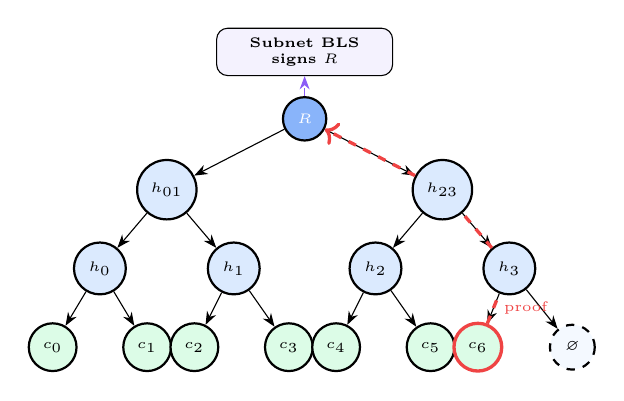
\begin{tikzpicture}[
  node distance=0.5cm and 0.5cm,
  mnode/.style={circle, draw, thick, minimum size=0.55cm, font=\tiny},
  leaf/.style={mnode, fill=lightgreen},
  inode/.style={mnode, fill=lightblue},
  root/.style={mnode, fill=icpblue!60, text=white, font=\tiny\bfseries},
  arr/.style={-Stealth},
  every node/.style={font=\tiny}
]
  \node[root]  (r)   at (3.5, 0)    {$R$};
  \node[inode] (n1)  at (1.75,-0.9) {$h_{01}$};
  \node[inode] (n2)  at (5.25,-0.9) {$h_{23}$};
  \node[inode] (n3)  at (0.9, -1.9) {$h_0$};
  \node[inode] (n4)  at (2.6, -1.9) {$h_1$};
  \node[inode] (n5)  at (4.4, -1.9) {$h_2$};
  \node[inode] (n6)  at (6.1, -1.9) {$h_3$};
  \node[leaf]  (l0)  at (0.3, -2.9) {$c_0$};
  \node[leaf]  (l1)  at (1.5, -2.9) {$c_1$};
  \node[leaf]  (l2)  at (2.1, -2.9) {$c_2$};
  \node[leaf]  (l3)  at (3.3, -2.9) {$c_3$};
  \node[leaf]  (l4)  at (3.9, -2.9) {$c_4$};
  \node[leaf]  (l5)  at (5.1, -2.9) {$c_5$};
  \node[leaf,draw=icpred,very thick] (l6) at (5.7,-2.9) {$c_6$};
  \node[leaf,fill=lightblue!30,dashed] (l7) at (6.9,-2.9){$\varnothing$};
  \draw[arr] (r)--(n1); \draw[arr] (r)--(n2);
  \draw[arr] (n1)--(n3); \draw[arr] (n1)--(n4);
  \draw[arr] (n2)--(n5); \draw[arr] (n2)--(n6);
  \draw[arr] (n3)--(l0); \draw[arr] (n3)--(l1);
  \draw[arr] (n4)--(l2); \draw[arr] (n4)--(l3);
  \draw[arr] (n5)--(l4); \draw[arr] (n5)--(l5);
  \draw[arr] (n6)--(l6); \draw[arr] (n6)--(l7);
  \draw[->, dashed, icpred, very thick]
    (l6) -- node[right, font=\tiny, icpred]{proof} (n6) -- (n2) -- (r);
  \node[draw, rounded corners, fill=lightpurple!60, minimum width=2.0cm,
        minimum height=0.5cm, font=\tiny\bfseries,
        text width=2.0cm, align=center] (bls)
       at (3.5, 0.85) {Subnet BLS signs $R$};
  \draw[arr, icppurple, dashed] (r) -- (bls);
\end{tikzpicture}
\caption{Merkle tree with 7 certificates. Adding leaf $c_6$ (red border) requires recomputing only 3 hashes (the dashed red path). Root $R$ is BLS-signed by the subnet.}
\label{fig:merkle}
\end{figure}

\subsection{Trustless Verification Protocol}

Verification requires \emph{no trust in the issuing institution}. Given a certificate and its Merkle proof $\pi$, the verifier performs five steps:

\begin{enumerate}
  \item \textbf{Hash check}: Recompute $h_c = \text{SHA-256}(\text{certificate fields})$ and confirm it matches the stored \texttt{certificate\_hash}.
  \item \textbf{Merkle proof walk}: Recompute the root from $h_c$ and the sibling hashes in $\pi$: $\hat{R} = \text{verifyProof}(h_c, \pi)$.
  \item \textbf{Fetch ICP certificate}: Request the ICP \emph{Certificate} (the BLS-signed state tree) from any ICP gateway node.
  \item \textbf{BLS signature check}: Verify the subnet's threshold BLS signature over the state tree root using the publicly known subnet key.
  \item \textbf{Root match}: Confirm that the canister's certified value in the state tree equals $\hat{R}$.
\end{enumerate}

The complete chain of trust can be expressed as:
\begin{equation}
  \text{fields} \xrightarrow{\text{SHA-256}} h_c \xrightarrow{\;\pi\;} \hat{R} \xrightarrow{\text{state tree}} \text{BLS sig} \xrightarrow{\text{subnet key}} \checkmark
\end{equation}

Steps 1--2 run entirely on the client side with no network call. Step 3 requires a single HTTP query to any ICP gateway (there is no need to contact the issuing university). The subnet public key is published by the DFINITY Foundation and can be independently verified via the on-chain Network Nervous System (NNS). No step requires trusting any single entity.

\subsection{Security Properties}

The following security properties follow directly from the construction:

\begin{itemize}[leftmargin=*]
  \item \textbf{Data integrity}: Any modification to a stored certificate changes its hash $h_c$, which breaks the Merkle proof and causes a root mismatch. This is detectable on the client side without contacting anyone.
  \item \textbf{Tamper-proof root}: The threshold BLS key is secret-shared across all subnet nodes. Forging a valid subnet signature requires compromising more than one-third of subnet nodes simultaneously — computationally and logistically infeasible across a geographically diverse, independently operated network.
  \item \textbf{Replay resistance}: Each certificate has a unique ID and a consensus-set nanosecond timestamp. Duplicate issuance attempts are rejected by the canister.
  \item \textbf{Unauthorized issuance prevention}: The \texttt{issueCertificate} function is gated by registered Ed25519 Principals. Forging access requires the university's private key.
  \item \textbf{Revocation freshness}: After a revocation, the Merkle root is updated within one consensus round (approximately 2 seconds), invalidating stale proofs far faster than traditional Certificate Revocation Lists.
  \item \textbf{Frontend integrity}: ICP's HTTP gateway signs canister asset responses via certified HTTP headers, making frontend tampering detectable in transit.
\end{itemize}

% =========================================================
\section{Implementation}
\label{sec:impl}

This section describes the technology stack, deployment details, and reproducibility information.

\subsection{Technology Stack}

\begin{itemize}[leftmargin=*]
  \item \textbf{Backend}: Written in Motoko, ICP's native programming language designed for canister development. Motoko provides orthogonal persistence (canister state survives upgrades automatically) and actor-based concurrency.
  \item \textbf{Frontend}: A React single-page application built with Vite. It includes three portals: a University Portal for issuance, a Student Portal for viewing credentials, and a Verification Portal for employers.
  \item \textbf{Candid Interface}: Auto-generated Candid bindings ensure type-safe communication between the JavaScript frontend and the Motoko backend.
  \item \textbf{Deployment}: Both canisters are deployed on ICP mainnet using the \texttt{dfx} CLI tool provided by DFINITY. The backend canister ID is \texttt{pekzw-diaaa-aaaad-afh3q-cai}.
\end{itemize}

\subsection{Canister Upgrade Safety}

ICP canisters can be upgraded without losing data, thanks to Motoko's \texttt{preupgrade} and \texttt{postupgrade} system hooks. Before an upgrade, the certificate map and Merkle state are serialized to stable storage. After the upgrade, they are deserialized and the Merkle tree is rebuilt from the stored certificates (a one-time O($n$) cost). This ensures that the certified root remains valid across upgrades.

\subsection{Key Code Paths}

Listing~\ref{lst:issue} shows the simplified issuance flow. The three key steps are: (1) verify that the caller is a registered university, (2) create the certificate record and compute its SHA-256 hash, and (3) insert the hash as a Merkle leaf and commit the new root via \texttt{CertifiedData.set()}.

\begin{lstlisting}[caption={Simplified issuance flow in Motoko},label={lst:issue},language={}]
public shared(msg) func issueCertificate(
    id: Text, name: Text, degree: Text, ...
) : async Text {
    // 1. Access control
    if (not isUniversity(msg.caller)) {
        return "Error: Unauthorized";
    };
    // 2. Create record and compute hash
    let cert = CertManager.createCertificate(
        id, name, degree, ...);
    certificates.put(id, cert);
    // 3. Incremental Merkle insert + certify
    insertCertLeaf(cert.certificate_hash);
    // insertCertLeaf internally calls:
    //   MerkleTree.insertLeaf(hash, state)  -- O(log n)
    //   CertifiedData.set(root_blob)        -- O(1)
    id
};
\end{lstlisting}

Listing~\ref{lst:verify} shows the verification flow. This is a \emph{query call} — it runs on a single replica, returns in under 500~ms, and costs nothing.

\begin{lstlisting}[caption={Simplified verification flow},label={lst:verify},language={}]
public query func verifyCertificate(
    id: Text) : async VerificationResult {
    switch (certificates.get(id)) {
        case null { ... "Not found" ... };
        case (?cert) {
            // O(log n) proof generation
            let proof = MerkleTree.getProof(
                cert.certificate_hash, state);
            // Client-side: walk proof to get root,
            // then verify BLS sig on state tree
            CertManager.verifyCertificate(
                cert, proof, merkleRoot);
        };
    };
};
\end{lstlisting}

The Merkle tree insertion (Listing~\ref{lst:insert}) places the new leaf at the next available position and recomputes only the path to the root — $\lceil\log_2 n\rceil$ hash operations.

\begin{lstlisting}[caption={Incremental Merkle leaf insertion},label={lst:insert},language={}]
public func insertLeaf(
    hash: Text, state: TreeState) : Text {
    let n = state.leaves.size();
    if (n >= state.cap) {
        // Double capacity and rebuild
        state.cap := state.cap * 2;
        state.nodes := Array.init(treeSize, EMPTY);
        placeLeaves(state);
        rebuildInternal(state);
    };
    state.leaves.add(hash);
    state.nodes[state.cap - 1 + n] := hash;
    // Walk up to root -- O(log n)
    var cur = state.cap - 1 + n;
    while (cur > 0) {
        let p = (cur - 1) / 2;
        state.nodes[p] := SHA256(
            state.nodes[2*p+1] # state.nodes[2*p+2]);
        cur := p;
    };
    state.nodes[0] // return new root
};
\end{lstlisting}

\subsection{Performance Monitoring}

The \texttt{PerformanceMetrics.mo} module records on-chain telemetry for every operation: start time, end time, duration, success/failure, and the current certificate count at the time of the operation. This data is used for canister-side monitoring. The last 1,000 metrics are kept in a buffer to prevent unbounded memory growth.

\subsection{Benchmark Suite}

We developed a dedicated Node.js benchmark suite using the \texttt{@dfinity/agent} library. The suite is configured in \texttt{benchmarks/suite/config.js} and measures:

\begin{itemize}[leftmargin=*]
  \item \textbf{Issuance}: Sequential and parallel issuance at batch sizes $n \in \{1, 10, 50, 100\}$, with 3 repetitions each.
  \item \textbf{Verification}: Sequential and concurrent queries at $n \in \{1, 10, 100, 500\}$.
  \item \textbf{Concurrent mixed workload}: Interleaved issuance (30\%) and verification (70\%) at concurrency levels $c \in \{1, 5, 10, 25, 50\}$.
  \item \textbf{Throughput}: Sustained 30-second sequential issuance, Merkle tree growth at different database sizes, and peak burst (100 simultaneous certificates).
  \item \textbf{Finality}: 20 independent update calls measuring time from submission to readable state.
\end{itemize}

A stable Ed25519 identity is used for all benchmark runs to ensure consistent authentication overhead.

\subsection{Reproducibility}

The complete source code, benchmark suite, and raw result JSON files are available in the project repository. All benchmarks were run against the live ICP mainnet canister in March 2026 from Bengaluru, India (approximately 50--80~ms round-trip time to ICP boundary nodes). Each experiment was repeated 3 times and we report mean, standard deviation, and percentiles (p50, p95, p99).

% =========================================================
\section{Experimental Evaluation}
\label{sec:eval}

All benchmarks were run against the live ICP mainnet canister \texttt{pekzw-diaaa-aaaad-afh3q-cai} in March 2026 using a Node.js benchmark suite (\texttt{@dfinity/agent}) from Bengaluru, India (approximately 50--80~ms round-trip time to ICP boundary nodes). Each experiment was repeated 3 times. We report mean, standard deviation, and percentiles (p50, p95, p99).

\subsection{Issuance Latency}

Table~\ref{tab:issuance} reports the wall-clock time and throughput for parallel issuance, where all $n$ certificates are submitted simultaneously. At $n = 1$, the wall time is approximately 1.9 seconds — the time for one consensus round. As the batch size increases, throughput grows because multiple certificates are processed across successive consensus rounds while the submissions overlap.

\begin{table}[t]
\caption{Parallel Issuance --- ICP Mainnet (3 trials each)}
\label{tab:issuance}
\centering\small\renewcommand{\arraystretch}{1.1}
\begin{tabular}{@{}crrrr@{}}
\toprule
\textbf{Batch ($n$)} & \textbf{Wall (ms)} & \textbf{p95 (ms)} & \textbf{Thpt (certs/s)} & \textbf{Stddev} \\
\midrule
1   & 1{,}943  & 2{,}111  & 0.52 & 143.6 \\
10  & 2{,}596  & 3{,}054  & 4.02 & 498.1 \\
50  & 6{,}933  & 7{,}320  & 7.23 & 325.2 \\
100 & 13{,}969 & 15{,}416 & 7.31 & 1{,}926.5 \\
\bottomrule
\end{tabular}
\end{table}

It is important to understand what happens during a parallel batch. All $n$ certificates are submitted at roughly the same instant, but the canister serializes update calls — only one update can be processed per consensus round. So the first certificate finishes in about 2 seconds, the second in about 4 seconds, and so on. For $n = 100$, the \emph{last} certificate finishes at about 14 seconds, but this does not mean each certificate takes 14 seconds — the canister was processing all 100 in a pipeline.

Fig.~\ref{fig:issuance_perc} shows the completion time percentiles for each batch size. At $n = 100$, the p50 (the time at which half the certificates are done) is about 10 seconds, and the p99 (the slowest certificate) is about 15 seconds.

\begin{figure}[t]
\centering
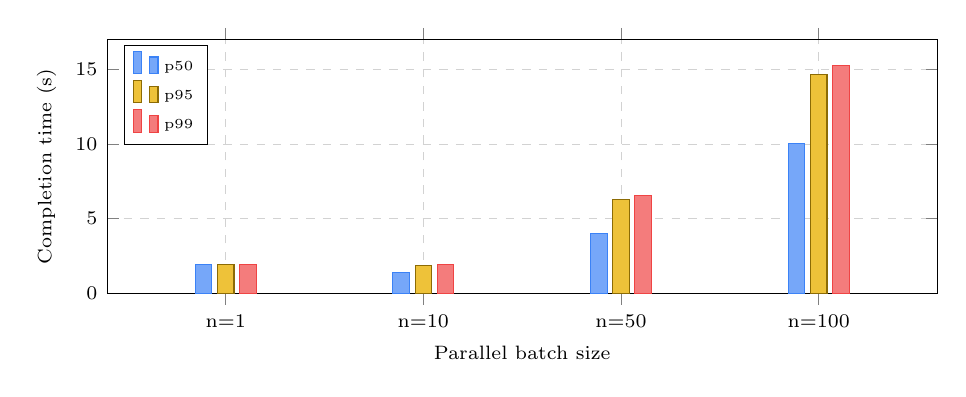
\begin{tikzpicture}
\begin{axis}[
  ybar, bar width=6pt,
  width=\columnwidth, height=4.8cm,
  symbolic x coords={n=1,n=10,n=50,n=100},
  xtick=data,
  xlabel={Parallel batch size},
  ylabel={Completion time (s)},
  ymin=0, ymax=17,
  enlarge x limits=0.2,
  grid=major, grid style={dashed,gray!35},
  legend style={at={(0.02,0.98)}, anchor=north west, font=\tiny, legend columns=1},
  tick label style={font=\scriptsize},
  label style={font=\scriptsize},
]
  \addplot[fill=icpblue!70,  draw=icpblue]
    coordinates {(n=1,1.91)(n=10,1.40)(n=50,4.00)(n=100,10.02)};
  \addlegendentry{p50}
  \addplot[fill=icpyellow!80, draw=icpyellow!60!black]
    coordinates {(n=1,1.91)(n=10,1.86)(n=50,6.31)(n=100,14.66)};
  \addlegendentry{p95}
  \addplot[fill=icpred!70,   draw=icpred]
    coordinates {(n=1,1.91)(n=10,1.90)(n=50,6.54)(n=100,15.28)};
  \addlegendentry{p99}
\end{axis}
\end{tikzpicture}
\caption{Parallel issuance completion time (p50/p95/p99). Each individual certificate takes about 1.9~s; the rising bars at large $n$ reflect queuing, not slower processing.}
\label{fig:issuance_perc}
\end{figure}

Table~\ref{tab:seq_issuance} shows the per-certificate latency when certificates are issued \emph{sequentially} (one at a time, waiting for each to finish before sending the next). The mean latency remains stable around 1.8--2.6 seconds regardless of how many certificates have already been issued, confirming that the Merkle tree's O($\log n$) insert cost does not degrade performance in practice.

\begin{table}[t]
\caption{Sequential Per-Certificate Issuance Latency (ms)}
\label{tab:seq_issuance}
\centering\small\renewcommand{\arraystretch}{1.1}
\begin{tabular}{@{}crrrrr@{}}
\toprule
\textbf{$n$} & \textbf{Mean} & \textbf{p50} & \textbf{p75} & \textbf{p95} & \textbf{p99} \\
\midrule
1   & 2{,}635 & 1{,}944 & 3{,}027 & 3{,}893 & 4{,}066 \\
10  & 2{,}077 & 1{,}914 & 2{,}079 & 4{,}227 & 5{,}050 \\
50  & 2{,}269 & 1{,}897 & 2{,}064 & 2{,}508 & 9{,}523 \\
100 & 1{,}821 & 1{,}861 & 1{,}982 & 2{,}257 & 3{,}561 \\
\bottomrule
\end{tabular}
\end{table}

\subsection{Verification Latency}

Verification is a \emph{query call} — it does not go through consensus and costs nothing to the caller. Table~\ref{tab:verif} and Fig.~\ref{fig:verif_perc} report verification latency against a live database of 500 certificates. The fastest observed query returned in \textbf{177~ms}, confirming that the Merkle proof computation adds negligible overhead. Even at 100 concurrent queries, the p99 remains below 1 second.

\begin{table}[t]
\caption{Verification Latency --- 500-Certificate Database (ms)}
\label{tab:verif}
\centering\small\renewcommand{\arraystretch}{1.1}
\begin{tabular}{@{}crrrrrr@{}}
\toprule
\textbf{Queries} & \textbf{Min} & \textbf{Mean} & \textbf{p50} & \textbf{p75} & \textbf{p95} & \textbf{p99} \\
\midrule
1   & 217 & 380 & 432 & 462 & 485 & 490 \\
10  & 177 & 518 & 512 & 578 & 722 & 980 \\
100 & --- & 491 & 498 & 567 & 787 & 994 \\
500 & --- & 485 & 477 & 563 & 693 & 924 \\
\bottomrule
\end{tabular}
\end{table}

\begin{figure}[t]
\centering
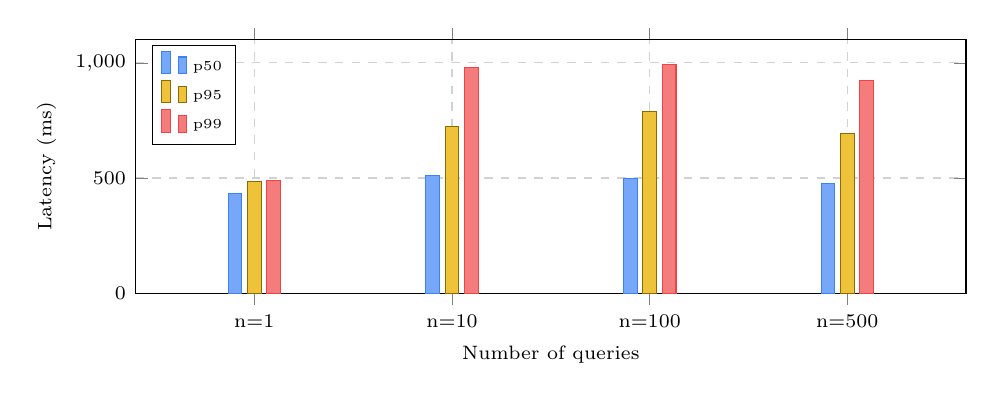
\begin{tikzpicture}
\begin{axis}[
  ybar, bar width=5pt,
  width=\columnwidth, height=4.8cm,
  symbolic x coords={n=1,n=10,n=100,n=500},
  xtick=data,
  xlabel={Number of queries},
  ylabel={Latency (ms)},
  ymin=0, ymax=1100,
  enlarge x limits=0.2,
  grid=major, grid style={dashed,gray!35},
  legend style={at={(0.02,0.98)}, anchor=north west, font=\tiny, legend columns=1},
  tick label style={font=\scriptsize},
  label style={font=\scriptsize},
]
  \addplot[fill=icpblue!70, draw=icpblue]
    coordinates {(n=1,432)(n=10,512)(n=100,498)(n=500,477)};
  \addlegendentry{p50}
  \addplot[fill=icpyellow!80, draw=icpyellow!60!black]
    coordinates {(n=1,485)(n=10,722)(n=100,787)(n=500,693)};
  \addlegendentry{p95}
  \addplot[fill=icpred!70, draw=icpred]
    coordinates {(n=1,490)(n=10,980)(n=100,994)(n=500,924)};
  \addlegendentry{p99}
\end{axis}
\end{tikzpicture}
\caption{Verification latency (p50/p95/p99) for 1 to 500 sequential queries. p99 stays below 1 second across all scales.}
\label{fig:verif_perc}
\end{figure}

\subsection{Throughput and Scalability}

An important question is whether throughput degrades as the database grows. To test this, we ran the issuance benchmark under two conditions: a fresh (low-count) database and a large database with approximately 3,280--3,461 existing certificates. Fig.~\ref{fig:throughput} shows the results.

\begin{figure}[t]
\centering
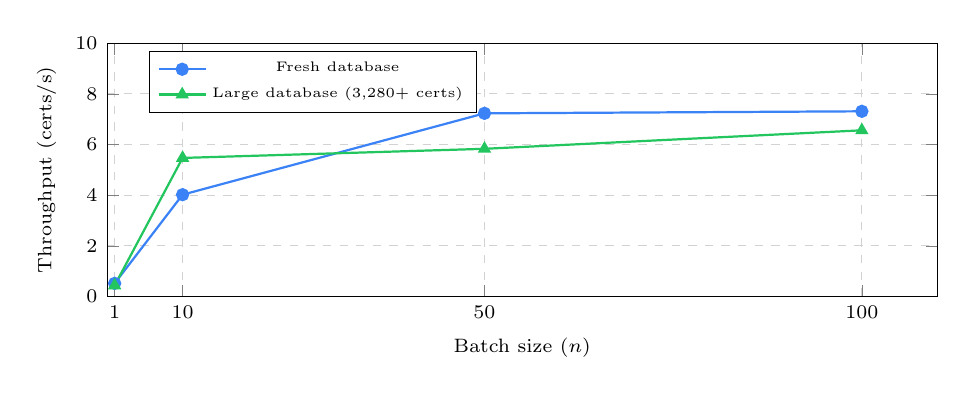
\begin{tikzpicture}
\begin{axis}[
  width=\columnwidth, height=4.8cm,
  xlabel={Batch size ($n$)},
  ylabel={Throughput (certs/s)},
  xmin=0, xmax=110,
  ymin=0, ymax=10,
  xtick={1,10,50,100},
  grid=both, grid style={dashed,gray!35},
  legend style={at={(0.05,0.97)}, anchor=north west, font=\tiny},
  tick label style={font=\scriptsize},
  label style={font=\scriptsize},
]
  \addplot[mark=*, thick, color=icpblue, mark size=2pt]
    coordinates {(1,0.52)(10,4.02)(50,7.23)(100,7.31)};
  \addlegendentry{Fresh database}
  \addplot[mark=triangle*, thick, color=icpgreen, mark size=2pt]
    coordinates {(1,0.44)(10,5.47)(50,5.83)(100,6.56)};
  \addlegendentry{Large database (3,280+ certs)}
\end{axis}
\end{tikzpicture}
\caption{Issuance throughput vs.\ batch size. The two curves track closely, confirming that the O($\log n$) Merkle insert cost does not degrade throughput as the database grows.}
\label{fig:throughput}
\end{figure}

The two curves nearly coincide: peak throughput is \textbf{7.3 certs/s} on a fresh database and \textbf{6.6 certs/s} on a large one — a difference of less than 10\%, confirming the O($\log n$) scalability claim.

\textbf{Sustained throughput}: Over a 30-second sequential issuance run, the system issued 17 certificates at a sustained rate of \textbf{0.57 certs/s} with mean latency 1,775~ms (p50: 1,847~ms, p95: 2,317~ms). The stable throughput with no degradation over time confirms that the canister does not suffer from memory pressure or garbage collection pauses during sustained operation.

\textbf{Peak burst}: 100 certificates submitted simultaneously all succeeded in 14,953~ms with \textbf{0\% error rate} (p50: 8,219~ms, p95: 14,158~ms, p99: 14,801~ms, mean: 8,261~ms).

\subsubsection{Merkle Tree Growth Impact}
To isolate the effect of database size on issuance latency, we measured batch wall-clock time at different database sizes. Table~\ref{tab:merkle_growth} shows the results.

\begin{table}[t]
\caption{Merkle Tree Growth --- Batch Wall-Clock Time}
\label{tab:merkle_growth}
\centering\small\renewcommand{\arraystretch}{1.1}
\begin{tabular}{@{}crrr@{}}
\toprule
\textbf{Batch ($n$)} & \textbf{Wall (ms)} & \textbf{DB Before} & \textbf{DB After} \\
\midrule
1   & 2{,}290  & 3{,}280 & 3{,}280 \\
10  & 1{,}828  & 3{,}281 & 3{,}291 \\
50  & 8{,}582  & 3{,}295 & 3{,}345 \\
100 & 15{,}234 & 3{,}361 & 3{,}461 \\
\bottomrule
\end{tabular}
\end{table}

Even with over 3,000 existing certificates, batch issuance times remain consistent with those measured on a fresh database (Table~\ref{tab:issuance}). This confirms that the O($\log n$) Merkle tree insert cost is not the bottleneck — consensus round time dominates.

\subsubsection{Concurrent Verification Throughput}
We also measured verification throughput when multiple queries are submitted simultaneously (Table~\ref{tab:conc_verif}).

\begin{table}[t]
\caption{Concurrent Verification Throughput}
\label{tab:conc_verif}
\centering\small\renewcommand{\arraystretch}{1.1}
\begin{tabular}{@{}crrr@{}}
\toprule
\textbf{Queries ($n$)} & \textbf{Wall (ms)} & \textbf{Queries/s} \\
\midrule
1   & 552   & 1.84 \\
10  & 629   & 15.97 \\
100 & 1{,}265 & 86.62 \\
\bottomrule
\end{tabular}
\end{table}

At 100 concurrent queries, the system achieves \textbf{86.6 queries/s} — well above what any realistic employer verification portal would need. The near-linear scaling demonstrates that query calls (which bypass consensus) scale efficiently on ICP.

\subsection{Concurrent Mixed Workload}

In a real-world deployment, the canister would receive issuance and verification requests simultaneously. The concurrent benchmark submits a mix of 30\% issuance (update) and 70\% verification (query) calls at increasing concurrency levels $c \in \{1, 5, 10, 25, 50\}$.

Fig.~\ref{fig:conc_tput} shows the total throughput (operations per second, counting both call types). Throughput grows from 0.55 ops/s at $c = 1$ to \textbf{13.59 ops/s} at $c = 50$ — a 25$\times$ speed-up with \textbf{zero errors} at all levels. The growth is sub-linear because issuance calls are serialized by consensus (one per round), while verification queries scale freely.

\begin{figure}[t]
\centering
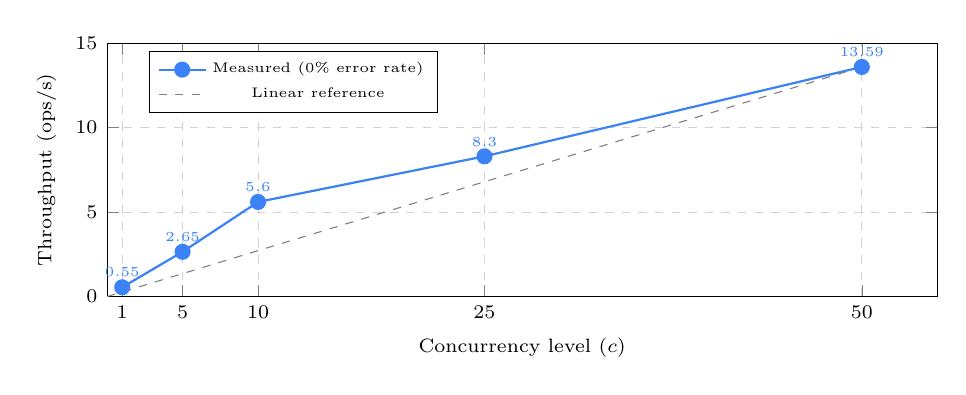
\begin{tikzpicture}
\begin{axis}[
  width=\columnwidth, height=4.8cm,
  xlabel={Concurrency level ($c$)},
  ylabel={Throughput (ops/s)},
  xmin=0, xmax=55,
  ymin=0, ymax=15,
  xtick={1,5,10,25,50},
  grid=both, grid style={dashed,gray!35},
  legend style={at={(0.05,0.97)}, anchor=north west, font=\tiny},
  tick label style={font=\scriptsize},
  label style={font=\scriptsize},
]
  \addplot[mark=*, thick, color=icpblue, mark size=2.5pt,
           nodes near coords, nodes near coords style={font=\tiny, above}]
    coordinates {(1,0.55)(5,2.65)(10,5.60)(25,8.30)(50,13.59)};
  \addlegendentry{Measured (0\% error rate)}
  \addplot[dashed, color=gray, no marks]
    coordinates {(0,0)(50,13.59)};
  \addlegendentry{Linear reference}
\end{axis}
\end{tikzpicture}
\caption{Mixed-workload throughput (30\% issue, 70\% verify). Sub-linear growth is because issuance calls are serialized per consensus round.}
\label{fig:conc_tput}
\end{figure}

Fig.~\ref{fig:conc_lat} breaks down the latency by operation type. Verification latency (query call, no consensus) remains stable between 565--847~ms across all concurrency levels. Issuance latency (update call, requires consensus) grows gradually from 1.7~s to 2.8~s as contention increases — a graceful degradation.

\begin{figure}[t]
\centering
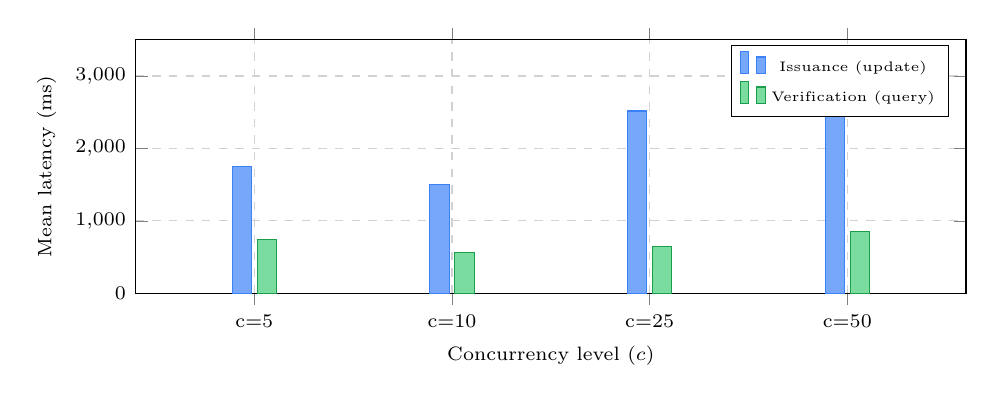
\begin{tikzpicture}
\begin{axis}[
  ybar, bar width=7pt,
  width=\columnwidth, height=4.8cm,
  symbolic x coords={c=5, c=10, c=25, c=50},
  xtick=data,
  xlabel={Concurrency level ($c$)},
  ylabel={Mean latency (ms)},
  ymin=0, ymax=3500,
  enlarge x limits=0.2,
  grid=major, grid style={dashed,gray!35},
  legend style={at={(0.98,0.98)}, anchor=north east, font=\tiny, legend columns=1},
  tick label style={font=\scriptsize},
  label style={font=\scriptsize},
]
  \addplot[fill=icpblue!70, draw=icpblue]
    coordinates {(c=5,1745)(c=10,1503)(c=25,2516)(c=50,2779)};
  \addlegendentry{Issuance (update)}
  \addplot[fill=icpgreen!60, draw=icpgreen!80!black]
    coordinates {(c=5,745)(c=10,565)(c=25,642)(c=50,847)};
  \addlegendentry{Verification (query)}
\end{axis}
\end{tikzpicture}
\caption{Latency by operation type. Verification stays under 850~ms even at $c = 50$. Issuance grows gradually due to consensus serialization.}
\label{fig:conc_lat}
\end{figure}

\subsection{Block Finality}

Block finality — the time from when a transaction is submitted until it is permanently committed and readable — was measured over 20 independent update calls. Table~\ref{tab:finality} summarizes the results.

\begin{table}[t]
\caption{Block Finality Time (20 samples)}
\label{tab:finality}
\centering\small\renewcommand{\arraystretch}{1.1}
\begin{tabular}{@{}lr@{}}
\toprule
\textbf{Metric} & \textbf{Value (ms)} \\
\midrule
Minimum   & 832 \\
Mean      & 2{,}356 \\
Std.\ Dev    & 421 \\
p50       & 2{,}395 \\
p75       & 2{,}622 \\
p95       & 2{,}811 \\
p99       & 2{,}944 \\
\bottomrule
\end{tabular}
\end{table}

The mean finality of \textbf{2.36 seconds} with a tight p99 of \textbf{2.94 seconds} confirms that ICP's consensus is fast and predictable. This makes TrustVault suitable for interactive use cases — an employer can verify a credential in real time during a job interview.

\subsection{Cross-Platform Comparison}

Table~\ref{tab:comparison} places TrustVault's measured performance alongside published benchmarks for Ethereum PoS and Hyperledger Fabric.

\begin{table*}[t]
\caption{Cross-Platform Comparison (all non-ICP values from cited literature)}
\label{tab:comparison}
\centering\small\renewcommand{\arraystretch}{1.2}
\begin{tabular}{@{}llll@{}}
\toprule
\textbf{Metric} & \textbf{ICP (TrustVault)} & \textbf{Ethereum PoS} & \textbf{Hyperledger Fabric} \\
\midrule
Block finality        & \textbf{2.36~s} (measured)    & $\approx$24~s~\cite{buterin2020eth2}  & $<$1~s~\cite{androulaki2018fabric} \\
Throughput            & 7.3 certs/s (measured)        & 15--30 TPS~\cite{dinh2017blockbench}  & $\approx$3{,}500 TPS~\cite{androulaki2018fabric} \\
Issuance cost         & \textbf{\$0.001} (measured)   & \$0.20--\$2.00~\cite{wood2014ethereum} & Near-zero \\
Verification cost     & \textbf{\$0} (query call)     & \$0.05--\$0.50~\cite{wood2014ethereum} & Near-zero \\
Frontend on-chain     & \textbf{Yes}                  & No                                     & No \\
Trust model           & \textbf{Zero-trust (BLS)}     & Zero-trust                             & Permissioned (consortium) \\
Data storage          & Full record on-chain          & Hash only (data off-chain)             & Full record on-chain \\
\bottomrule
\end{tabular}
\end{table*}

Key observations:
\begin{itemize}[leftmargin=*]
  \item ICP's finality (2.36~s) is about 10$\times$ faster than Ethereum PoS (24~s) but slower than Fabric ($<$1~s). However, Fabric requires trusting the consortium.
  \item ICP's per-credential cost (\$0.001) is 200--2{,}000$\times$ cheaper than Ethereum.
  \item TrustVault is the only system where both the verification result and the verification \emph{interface} are served from the blockchain itself.
  \item Fabric achieves far higher raw throughput (3{,}500 TPS), but this is for a permissioned network where all validators are known and trusted — a fundamentally different security model.
\end{itemize}

% =========================================================
\section{Discussion}
\label{sec:discussion}

This section discusses the practical implications, limitations, and trade-offs of our approach.

\subsection{Practical Suitability}

The benchmark results demonstrate that TrustVault is practical for real-world use. Consider a mid-sized university that graduates 5,000 students per year. At 7.3 certs/s parallel throughput, all credentials could be issued in approximately 11 minutes. At \$0.001 per credential, the total annual issuance cost would be about \$5 — negligible compared to the cost of maintaining a traditional verification office.

For employers, verification queries return in under 500~ms (median) and are completely free. An employer portal could verify hundreds of candidates per minute without any cost or rate-limiting concern.

The 2.36-second finality means that a freshly issued credential becomes verifiable within about 3 seconds of issuance — fast enough for interactive use cases such as verifying a credential during a live interview.

\subsection{Limitations}

\subsection{Throughput Ceiling}
TrustVault's parallel throughput plateaus at approximately 7.3 certs/s because ICP serializes update calls within a single canister — only one update can be processed per consensus round (approximately 2 seconds). This is a fundamental property of ICP's consensus model: each canister processes state-mutating calls sequentially to guarantee consistency.

For a single university, this throughput is more than sufficient — even a large university issuing 50,000 credentials annually could process all of them in under 2 hours. For a national-scale system handling millions of credentials simultaneously, a multi-canister sharding architecture would be necessary. In such an architecture, credentials would be distributed across multiple backend canisters (e.g., one per state or region), each maintaining its own Merkle tree. A coordinator canister could aggregate the individual Merkle roots into a global root for cross-canister verification.

\subsubsection{Revocation Cost}
Revoking a certificate currently triggers a full O($n$) Merkle tree rebuild because the tree structure must be recomputed without the revoked leaf. For a database of 10,000 certificates, this adds approximately 1--2 seconds of additional latency. An optimization would be to use a ``soft revocation'' approach — marking the certificate's \texttt{is\_revoked} field as \texttt{true} and rebuilding only the affected path. Alternatively, a cryptographic accumulator (e.g., RSA accumulator) could support both insertion and deletion in O(1) time, though with larger proof sizes. We leave this exploration to future work.

\subsubsection{Network Latency}
Our benchmarks were run from India (50--80~ms RTT to ICP boundary nodes). Users closer to boundary nodes (e.g., in the US or Europe) would see lower absolute latencies. Conversely, users in regions with high network latency would see proportionally higher latencies for both the network round-trip and the consensus wait.

\subsubsection{ICP Platform Dependency}
TrustVault is built on ICP and relies on the ICP subnet infrastructure. If the DFINITY Foundation or the NNS governance system were to make breaking changes to the platform, the canister might need to be updated. However, ICP's governance is decentralized (proposals require community approval via NNS voting), and canisters can be made ``blackholed'' (immutable) if desired — at the cost of giving up upgradeability.

\subsubsection{Hash-Based Verification}
The current certificate hash is computed from core identity fields. If two students have identical names, IDs, degree types, majors, and graduation dates (an unlikely but theoretically possible collision), their hashes could collide. In practice, the unique \texttt{certificate\_id} field removes this risk.

\subsection{Comparison with W3C Verifiable Credentials}

TrustVault's certificate schema is not currently compatible with the W3C Verifiable Credentials data model~\cite{w3c2022vc}. However, the W3C VC standard defines a flexible JSON-LD format that can represent any credential type. Wrapping TrustVault's certificate records in a W3C VC envelope — with the ICP BLS signature serving as the cryptographic proof — would enable interoperability with other VC-compatible systems. We plan to add this in a future version.

\subsection{Privacy Considerations}

TrustVault stores credential data on a public blockchain, which means that anyone can query the canister to look up credentials by student ID or university name. While this is the intended behavior for a verification system (the whole point is that anyone can verify), it may raise privacy concerns in jurisdictions with strict data protection laws (e.g., GDPR). A privacy-preserving extension could use zero-knowledge proofs to allow verification without revealing the full credential details — for example, proving ``this person holds a Bachelor's degree from university X'' without revealing their GPA or exact graduation date. We consider this an important direction for future work.

\subsection{Deployment Experience}

Deploying TrustVault on ICP mainnet involved the following steps:

\begin{enumerate}
  \item \textbf{Local development}: The canister was developed and tested locally using the \texttt{dfx} CLI tool, which provides a local ICP replica for testing.
  \item \textbf{Cycle acquisition}: ICP tokens were purchased and converted to cycles using the NNS dApp. Approximately 4 trillion cycles (about \$5) were allocated for deployment and initial operation.
  \item \textbf{Mainnet deployment}: The backend and frontend canisters were deployed to the ICP mainnet using \texttt{dfx deploy --network ic}. Each canister received a unique canister ID.
  \item \textbf{University registration}: The deployer's Principal was registered as a university, allowing it to issue test credentials.
  \item \textbf{Benchmarking}: The benchmark suite was run from a separate machine in Bengaluru, India, using a dedicated Ed25519 identity.
\end{enumerate}

The entire deployment process took approximately 30 minutes and cost less than \$5 in cycles. The canister has been running continuously on mainnet since deployment with no downtime or maintenance required.

\subsection{Scalability Projections}

Based on our measured throughput of 7.3 certs/s (parallel) and 0.57 certs/s (sustained sequential), we can project the following capacity:

\begin{itemize}[leftmargin=*]
  \item \textbf{Small university} (1,000 graduates/year): All credentials could be issued in 2.3 minutes (parallel) at a cost of \$1.
  \item \textbf{Large university} (50,000 graduates/year): All credentials could be issued in 1.9 hours (parallel) at a cost of \$50.
  \item \textbf{National system} (1 million graduates/year): With a single canister, issuance would take about 38 hours. With 10 canisters (multi-canister sharding), this drops to under 4 hours at a cost of approximately \$1,000.
  \item \textbf{Verification load}: At 86.6 queries/s, a single canister can handle over 7.4 million verification queries per day — more than enough for any realistic deployment.
\end{itemize}

These projections assume current ICP subnet performance. As ICP adds more subnets and optimizes consensus, these numbers are expected to improve over time.

% =========================================================
\section{Conclusion and Future Work}
\label{sec:conclusion}

This paper presented TrustVault, a fully on-chain academic credential verification system built on the Internet Computer Protocol. TrustVault stores both the credential data and the end-user verification interface on the blockchain, eliminating every centralized point of failure. By combining an incremental binary Merkle tree with ICP's Certified Variables (threshold BLS-signed state), TrustVault enables \emph{trustless} verification: a verifier who knows only the ICP subnet public key can independently confirm any credential without contacting the issuing institution.

Our comprehensive benchmarks on the live ICP mainnet demonstrate practical performance:
\begin{itemize}[leftmargin=*]
  \item Single-certificate issuance in approximately 1.9 seconds.
  \item Verification queries as fast as 177~ms (free of charge).
  \item Parallel throughput up to 7.3 certificates per second.
  \item Concurrent mixed-workload throughput of 13.6 ops/s with zero errors.
  \item Block finality of 2.36 seconds (p99 under 3 seconds).
  \item Issuance cost of approximately \$0.001 per certificate.
  \item O($\log n$) Merkle tree scaling confirmed with less than 10\% throughput difference between a fresh and a 3,400-certificate database.
\end{itemize}

Compared to Ethereum PoS, TrustVault is 10$\times$ faster in finality and 200--2{,}000$\times$ cheaper per credential. Compared to Hyperledger Fabric, TrustVault provides true zero-trust verification without requiring trust in a consortium.

\subsection{Future Work}

Several directions for future work are planned:

\begin{enumerate}
  \item \textbf{W3C Verifiable Credentials integration}: Wrapping TrustVault credentials in the W3C VC JSON-LD format would enable interoperability with other credential systems worldwide. The ICP BLS signature would serve as the cryptographic proof within the VC envelope.
  \item \textbf{Multi-canister sharding}: Distributing credentials across multiple canisters (one per region or institution) would break the single-canister throughput ceiling and enable national-scale deployments.
  \item \textbf{Internet Identity integration}: ICP's Internet Identity system provides a passwordless, privacy-preserving authentication mechanism based on WebAuthn/FIDO2. Integrating it would allow students and universities to authenticate using biometrics (fingerprint, Face ID) instead of managing private keys.
  \item \textbf{Zero-knowledge proofs for selective disclosure}: Using ZK-SNARKs or ZK-STARKs, a credential holder could prove specific facts (``I hold a degree from university X'') without revealing other fields (GPA, exact dates). This would address privacy concerns while maintaining the trustless verification property.
  \item \textbf{Mobile SDK}: A lightweight library for verifying credentials directly from a mobile app, using the ICP agent protocol to communicate with boundary nodes.
  \item \textbf{Batch revocation optimization}: Replacing the full O($n$) tree rebuild with accumulator-based revocation or incremental tree surgery to reduce revocation latency.
  \item \textbf{Cross-subnet scalability testing}: Deploying canisters across multiple ICP subnets and measuring inter-canister call overhead for a sharded architecture.
\end{enumerate}

% =========================================================
\section*{Acknowledgments}
The authors thank the DFINITY Foundation for maintaining the Internet Computer Protocol infrastructure and providing public documentation. Benchmark testing used ICP mainnet cycles funded by the authors.

% =========================================================
\balance
\begin{thebibliography}{99}

\bibitem{chahal2021credential}
H.~Chahal and S.~Singh,
``Credential fraud in South Asia: Findings and implications for the higher education sector,''
\textit{International Journal of Educational Management}, vol.~35, no.~7, pp.~1498--1512, 2021.

\bibitem{buterin2014ethereum}
V.~Buterin,
``A next-generation smart contract and decentralized application platform,''
Ethereum White Paper, 2014.
[Online]. Available: \url{https://ethereum.org/whitepaper}

\bibitem{androulaki2018fabric}
E.~Androulaki \textit{et al.},
``Hyperledger Fabric: A distributed operating system for permissioned blockchains,''
in \textit{Proc.\ EuroSys'18}, 2018, pp.~1--15.

\bibitem{hanke2018dfinity}
T.~Hanke, M.~Movahedi, and D.~Williams,
``DFINITY Technology Overview Series, Consensus System,''
\textit{arXiv:1805.04548}, 2018.

\bibitem{boneh2001bls}
D.~Boneh, B.~Lynn, and H.~Shacham,
``Short signatures from the Weil pairing,''
in \textit{ASIACRYPT 2001}, LNCS vol.~2248, pp.~514--532, 2001.

\bibitem{dfinity2022geeks}
DFINITY Foundation,
``The Internet Computer for Geeks,''
White Paper, 2022.
[Online]. Available: \url{https://internetcomputer.org/whitepaper.pdf}

\bibitem{merkle1989certified}
R.~C.~Merkle,
``A certified digital signature,''
in \textit{CRYPTO'89}, LNCS vol.~435, pp.~218--238, 1989.

\bibitem{grech2017blockchain}
J.~Grech and A.~F.~Camilleri,
``Blockchain in Education,''
EUR 28778 EN, Publications Office of the European Union, Luxembourg, 2017.

\bibitem{turk2018eductx}
M.~Turkanovi\'{c}, M.~H\"{o}lbl, K.~Ko\v{s}i\v{c}, M.~Heri\v{c}ko, and A.~Kami\v{s}ali\'{c},
``EduCTX: A blockchain-based higher education credit platform,''
\textit{IEEE Access}, vol.~6, pp.~5112--5127, 2018.

\bibitem{lizcano2020blockchain}
D.~Lizcano, J.~A.~Lara, B.~White, and S.~Aljawarneh,
``Blockchain-based approach to create a model of trust in open and ubiquitous higher education,''
\textit{Journal of Computing in Higher Education}, vol.~32, pp.~109--134, 2020.

\bibitem{w3c2022vc}
M.~Sporny, D.~Longley, and D.~Chadwick,
``Verifiable Credentials Data Model v1.1,''
W3C Recommendation, Mar.~2022.
[Online]. Available: \url{https://www.w3.org/TR/vc-data-model/}

\bibitem{wood2014ethereum}
G.~Wood,
``Ethereum: A secure decentralised generalised transaction ledger,''
Ethereum Yellow Paper, 2014.

\bibitem{buterin2020eth2}
V.~Buterin, D.~Hernandez, T.~Kamphefner, K.~Pham, Z.~Qiao, D.~Ryan, J.~Sin, Y.~Wang, and Y.~X.~Zhang,
``Combining GHOST and Casper,''
\textit{arXiv:2003.03052}, 2020.

\bibitem{dinh2017blockbench}
T.~T.~A.~Dinh, R.~Fan, G.~Wang, and B.~C.~Ooi,
``BLOCKBENCH: A framework for analyzing private blockchains,''
in \textit{Proc.\ ACM SIGMOD}, 2017, pp.~1085--1100.

\bibitem{sharmaperformance2019}
A.~Sharma, F.~M.~Schuhknecht, D.~Agrawal, and J.~Dittrich,
``Blurring the lines between blockchains and database systems: the case of Hyperledger Fabric,''
in \textit{Proc.\ ACM SIGMOD}, 2019, pp.~105--122.

\bibitem{camenisch2001efficient}
J.~Camenisch and A.~Lysyanskaya,
``An efficient system for non-transferable anonymous credentials with optional anonymity revocation,''
in \textit{EUROCRYPT 2001}, LNCS vol.~2045, pp.~93--118, 2001.

\bibitem{allen2016decentralized}
C.~Allen,
``The path to self-sovereign identity,''
\textit{Life With Alacrity blog}, Apr.~2016.
[Online]. Available: \url{http://www.lifewithalacrity.com/2016/04/the-path-to-self-soverereign-identity.html}

\bibitem{gipp2015decentralized}
B.~Gipp, N.~Meuschke, and A.~Gernandt,
``Decentralized trusted timestamping using the crypto currency Bitcoin,''
in \textit{Proc.\ iConference}, 2015, pp.~1--6.

\bibitem{nzaou2022credential}
A.~Nzaou, P.~Fabian, and M.~Samwel,
``Blockchain-based academic credential verification: A systematic review,''
\textit{Education and Information Technologies}, vol.~27, pp.~9503--9540, 2022.

\bibitem{dfinity2023httpgateway}
DFINITY Foundation,
``HTTP Gateway Protocol Specification,''
2023.
[Online]. Available: \url{https://internetcomputer.org/docs/references/http-gateway-protocol-spec}

\end{thebibliography}

\end{document}
